\section{Requirements)}
\section{Model and Dataset Selection}
\section{Concept and design}
\subsection{GUI Application}
\subsection{Validation and Benchmarking Pipeline}
\subsection{Performance Evaluation (CPU vs GPU)}
\subsection{Custom Dataset Integration}







Here is a sentence, and you can see a nice picture in Figure \ref{fig:duck}. You can also use the \kbd{autoref} command to do this automatically, like this:~\autoref{fig:duck}.

\begin{figure}[h]
    \centering
    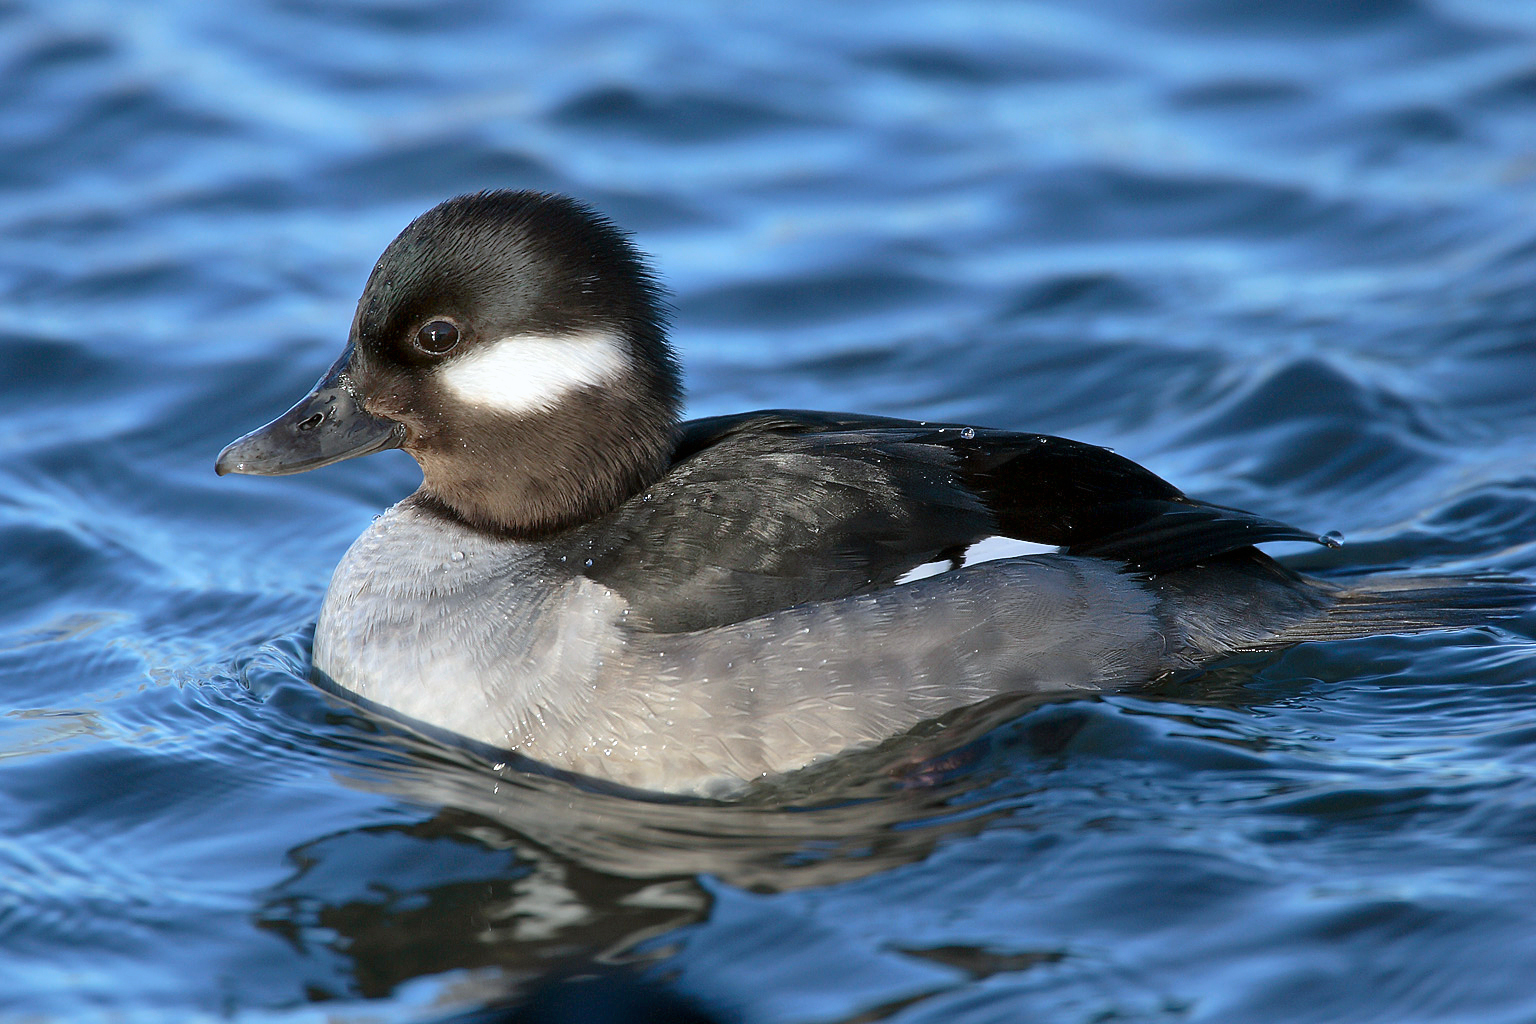
\includegraphics[width=\linewidth]{figures/duck.jpg}
    \caption{A picture of a duck.}
    \label{fig:duck}
\end{figure}

Also, a table can be found in Table \ref{tbl:example-table}. You should use a \LaTeX~table generator like \url{https://www.tablesgenerator.com/} if you want to make your life easier.

\begin{table}[h]
    \caption{Here is a table. The caption goes above like this.}
    \centering
    \begin{tabular}{l|l|c}
        First name & Last name & Age \\
        \hline\hline
        Bob & Bobbington & 24 \\
        Benth & Wavies & 49 \\
        Joe & Bloggs & 37 \\
        Billy & Bob & 10 \\

    \end{tabular}
    \label{tbl:example-table}
\end{table}